\documentclass{article}

\usepackage{amsmath, amssymb}
\usepackage{array}
\usepackage[a3paper, margin=1in]{geometry}
%% landscape
\usepackage{tikz}
\usetikzlibrary{arrows}
\tikzset{
every picture/.style={very thick}
}

%%font
\usepackage{euler}
\usepackage[OT1]{eulervm}
\renewcommand{\rmdefault}{pplx}

\newcommand{\Var}{\operatorname{Var}}

\tikzset{
  g5/.pic={
    \foreach \i in {1,2,...,5} {
      \pgfmathsetmacro{\ang}{90 + 72*(\i - 1)}
      \node[draw, circle, inner sep=2pt] (\i) at (\ang:2) {};
    }
    \draw[dashed] (1) -- (2) -- (3) -- (4) -- (5) -- (1);
    \draw[dashed] (3) -- (1) -- (4);
  }
}

\begin{document}
%% absolute positioning
%% \begin{tikzpicture}[remember picture, overlay]
%%   \draw ([xshift=\x]current page.south) -- ([xshift=\x]current page.north);
%% \end{tikzpicture}    

\pagenumbering{gobble}

For each graph, add as many edges as possible so that they do not create any cycles---such a structure is called a \emph{spanning tree}.

\begin{center}
  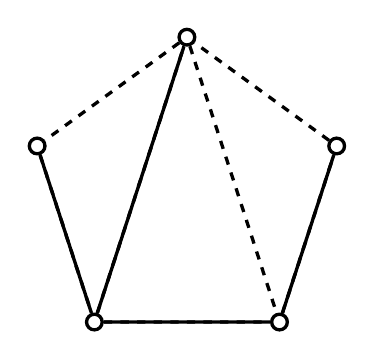
\begin{tikzpicture}
    \foreach \i in {1,2,...,5} {
      \pgfmathsetmacro{\ang}{90 + 72*(\i - 1)}
      \node[draw, circle, inner sep=2pt] (\i) at (\ang:2) {};
    }
    \draw[dashed] (1) -- (2) -- (3) -- (4) -- (5) -- (1);
    \draw[dashed] (3) -- (1) -- (4);
    \draw (2) -- (3) -- (4) -- (5);
    \draw (1) -- (3);
  \end{tikzpicture}
  \hfil
  \tikz\pic at (0,0) {g5};
  \hfil
  \tikz\pic at (0,0) {g5};
  \hfil
  \tikz\pic at (0,0) {g5};
  \hfil
  \tikz\pic at (0,0) {g5};
\end{center}

\begin{center}
  \tikz\pic at (0,0) {g5};
  \hfil
  \tikz\pic at (0,0) {g5};
  \hfil
  \tikz\pic at (0,0) {g5};
  \hfil
  \tikz\pic at (0,0) {g5};
  \hfil
  \tikz\pic at (0,0) {g5};
\end{center}

\begin{center}
  \tikz\pic at (0,0) {g5};
  \hfil
  \tikz\pic at (0,0) {g5};
  \hfil
  \tikz\pic at (0,0) {g5};
  \hfil
  \tikz\pic at (0,0) {g5};
  \hfil
  \tikz\pic at (0,0) {g5};
\end{center}

\begin{center}
  \tikz\pic at (0,0) {g5};
  \hfil
  \tikz\pic at (0,0) {g5};
  \hfil
  \tikz\pic at (0,0) {g5};
  \hfil
  \tikz\pic at (0,0) {g5};
  \hfil
  \tikz\pic at (0,0) {g5};
\end{center}

\begin{center}
  \tikz\pic at (0,0) {g5};
  \hfil
  \tikz\pic at (0,0) {g5};
  \hfil
  \tikz\pic at (0,0) {g5};
  \hfil
  \tikz\pic at (0,0) {g5};
  \hfil
  \tikz\pic at (0,0) {g5};
\end{center}

Number of spanning trees $=$

\vspace{2cm}

\begin{center}

  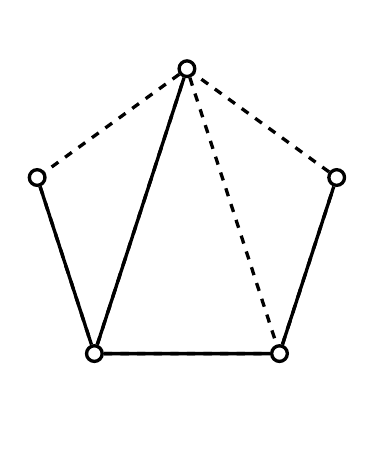
\begin{tikzpicture}
    \foreach \i in {1,2,...,5} {
      \pgfmathsetmacro{\ang}{90 + 72*(\i - 1)}
      \node[draw, circle, inner sep=2pt] (\i) at (\ang:2) {};
    }
    \draw[dashed] (1) -- (2) -- (3) -- (4) -- (5) -- (1);
    \draw[dashed] (3) -- (1) -- (4);
    \draw (2) -- (3) -- (4) -- (5);
    \draw (1) -- (3);
    \draw[opacity=0](0,-2.5) -- (0,2.5);
  \end{tikzpicture}
  \hfil
  \begin{tikzpicture}
    \draw[-triangle 45] (-2,0) -- (2,0);
    \node[rectangle, draw=none] at (0,0.5) {Laplacian matrix};
    \draw[opacity=0](0,-2.5) -- (0,2.5);
  \end{tikzpicture}
  \hfil
  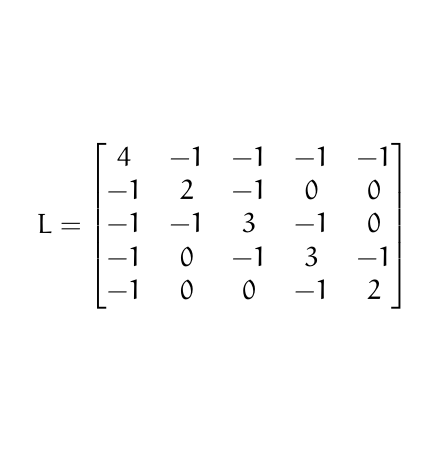
\begin{tikzpicture}
    \node[draw=none, rectangle] at (0,0) {
      $L = \begin{bmatrix}
        4 & -1 & -1 & -1 & -1 \\
        -1 & 2 & -1 & 0 & 0 \\
        -1 & -1 & 3 & -1 & 0 \\
        -1 & 0 & -1 & 3 & -1 \\
        -1 & 0 & 0 & -1 & 2 \\
      \end{bmatrix}$
    };
    \draw[opacity=0](0,-2.5) -- (0,2.5);
  \end{tikzpicture}
  \hfil
  \begin{tikzpicture}
    \draw[-triangle 45] (-2,0) -- (2,0);
    \node[rectangle, draw=none] at (0,0.5) {remove $1$st row/column};
    \draw[opacity=0](0,-2.5) -- (0,2.5);
  \end{tikzpicture}
  \hfil
  \begin{tikzpicture}
    \node[draw=none, rectangle] at (0,0) {
      $L(1) = \begin{bmatrix}
        2 & -1 & 0 & 0 \\
        -1 & 3 & -1 & 0 \\
        0 & -1 & 3 & -1 \\
        0 & 0 & -1 & 2 \\
      \end{bmatrix}$
    };
    \draw[opacity=0](0,-2.5) -- (0,2.5);
  \end{tikzpicture}  
\end{center}

$\det(L(1)) =$

\end{document}

